\documentclass[10pt]{article}

%---------------------------------------------------------------------

\usepackage[a4paper, headsep=0in,bindingoffset=0in,%
left=0.7in,right=0.7in,top=0.7in,bottom=0.7in,%
footskip=.25in]{geometry}

\usepackage[english]{babel}   
\usepackage[utf8]{inputenc}  
\usepackage{sectsty}
\usepackage{subcaption}


\usepackage{graphicx}
\usepackage[
backend=bibtex,
style=numeric,
sorting=none
]{biblatex}
\addbibresource{feb25bib.bib}
\usepackage{amsfonts}
\graphicspath{{/Users/emilyolafson/GIT/stroke-graph-matching/apaper/figs/}}

\renewcommand{\baselinestretch}{1.3}
\usepackage{verbatim}
\usepackage{listings}
\usepackage{indentfirst}
\setlength{\parindent}{1cm}
%\setlength{\parskip}{0.5cm}

\setlength{\headsep}{1pt}
%---------------------------------------------------------------------

\begin{document} 
	\sectionfont{\large}
	\title{Functional connectome reorganization after pontine stroke is associated with better motor  	outcomes}
	\maketitle
 	\author{Emily Olafson, Keith Jamison, Hesheng Liu, Danhong Wang, Joel Bruss, Aaron Boes, Amy Kuceyeski}%, Keith Jamison, PhD\inst{1}, Hesheng Liu, MD\inst{2}, Danhong Wang, MD\inst{2},Joel Bruss, PhD\inst{3}, Aaron Boes, MD PhD\inst{3}, Amy Kuceyeski, PhD\inst{1}}
	% E-MAILS
	%\address{Weill Cornell Medical College, \inst{2} Harvard Medical School, \\ \inst{3}Massachusetts General Hospital, \inst{4}University of Iowa 
	%}
	
	%---------------------------------------------------------------------
	\section*{Introduction}
	Motor deficits are the most common and disruptive symptoms of ischemic stroke, but spontaneous recovery of motor function occurs for most patients \cite{Duncan2000-uj}. This motor recovery is dependent on the ability of brain networks to functionally reorganize and compensate for lost brain areas \cite{Corbetta2005-ra}. As demonstrated by animal models, the functional role of motor regions damaged by stroke may be adopted by surviving tissue around the site of the lesion, but brain areas distant to the damaged tissue with similar function and connectivity as the lesion site have also been shown to compensate for lost function in animals, typically when the initial infarct is large \cite{Winship2009-af, Adam2020-jk, Murata2015-ss, Brown2009-jn}.
	\\
	
	In humans, functional reorganization underlying post-stroke motor recovery has been studied with resting-state functional magnetic resonance imaging (fMRI). Strong evidence suggests that crucial to eventual motor recovery is the restoration of interhemispheric resting-state functional connectivity (FC) between the primary motor cortices \cite{Carter2010-er, Urbin2014-iq, Rehme2013-ap}, but less is known about how the brain’s functional networks change on a greater spatial and temporal scale after stroke. Altered network topology \cite{Wang2010-or} and recruitment of other networks aside from the motor network such as the frontoparietal network \cite{Hordacre2021-ct, Pool2018-px} have been implicated in the recovery process, but network changes at a high temporal resolution have not been well documented.
	\\
	
	Prior studies investigating neural correlates of motor recovery have focused almost exclusively on supratentorial strokes that impact the internal capsule and surrounding areas. Evidence suggests that for pontine strokes, which impact the  connections between motor cortex and the cerebellu \cite{Lu2011-ow}, and account for roughly 7 percent of all ischemic strokes \cite{Saia2009-ik} sources of motor deficits as well as recovery-related reorganization might differ from those of supratentorial strokes. Reduced blood flow as measured by arterial spin labeling has been observed in the cerebellum and cortical regions in pontine stroke \cite{Wei2020-gj, Wang2019-jr} and longitudinally, changes in cerebral blood flow in cortical areas including the supramarginal gyrus and middle occipital gyrus were related to motor recovery. Areas with abnormal blood flow over time also had abnormal FC \cite{Wei2020-gj}, and increased degree centrality in the ipsilesional cerebellum has been related to better motor recovery \cite{Liu2019-mj}. The network changes associated with functional damage and subsequent recovery in pontine stroke have yet to be assessed in a longitudinal study.
	\\
	
	Secondary damage due to diaschisis, which affects remote brain areas anatomically connected to the lesion, results in widespread disruption of functional networks \cite{Carrera2014-ah}. Functional impairment and subsequent reorganization of areas anatomically connected to the lesion may be an important component of the recovery process that has yet to be explored. In this study, we propose a novel measure to capture adaptive functional plasticity after pontine stroke, outlined below, and connect it to patterns of structural disruption after stroke. 
	\\
	
	Connectivity to the rest of the brain is one aspect of a brain region's functional role in the network. We propose that instances of functional reorganization over time, as in the case of adjacent surviving tissue adopting the functional role of lost tissue, may be captured by identifying brain regions whose pattern of FC with the rest of the brain is more closely matched by a different brain region at a later date. Considering functional connectomes as graph, the task of identifying similar nodes (gray matter regions, in this case) between two functional connectomes can be considered a graph matching problem \cite{Conte2004-ro}. Graph matching has been applied recently to map individual structural connectomes to their functional connectomes \cite{Osmanlioglu2019-ao}. Conceptually, the process of graph matching exchanges the labels of nodes when doing so results increased similarity of the two networks. When two regions exchange FC profiles, the regions are said to have been ‘remapped’. We hypothesize that brain regions with more structural damage due to the lesion will more frequently functionally reorganize; that more impaired subjects will have more global functional reorganization; and that the amount of functional reorganization will correlate with the change in motor impairment between subsequent sessions.
	

	\section*{Methods} \label{sec:firstpage}
	
	\subsubsection*{Data description}
	 Twenty-three first-episode stroke patients (x-y years old; mean age, X years; x male, x right-handed) with isolate pontine infarcts. X subject had right pontine infarcts, Y had left infarcts, U had bilateral and is described previously (Supplementary Fig) \cite{Lu2011-ow}. Patient were scanned five times during a period of 6 months (7, 14, 30, 90 and 180 days after stroke onset, on a 3T TimTrio Siemens using a 12-channel phase-array head coil. Structural images were acquired using a sagittal MP-RAGE three-dimensional T1-weighed sequence (TR, 1600ms; TE 2.15ms; flip angle, 9°, 1.0 mm isotropic voxels (FOV, 256 x 256). Each MRI session involved two to four runs (360s each run) of resting-state fMRI. Subjects were instructed to stay awake and keep their eyes open; no other task instruction was provided. Images were acquired using the gradient-echo echo-planar pulse sequence (TR, 3000ms; TE, 30ms; flip angle, 90°, 3 mm isotropic voxels).
	
	\subsubsection*{Structural data processing}
	Preprocessing of the longitudinal structural data included registration of each subject’s session 2-5 T1 scans to the space of session 1, collapsing co-registered files to an average, creation of a skull-stripped brain mask, followed by manual editing and binarization of the hand-edited mask. Each mask was then pushed to each of the session 2-5 T1s in native space using the inverse registration acquired from the first step. This was followed by bias field correction of the 5 T1 scans, transformation of native-space bias field-corrected data back to session 1 space, and the creation of an average bias field-corrected scan for each subject. Lesion masks were hand-drawn on these transformed T1 scans by ADB and JEB.
	
	\subsubsection*{Functional data processing}
	Preprocessing of the longitudinal functional data was performed using the CONN toolbox, including functional realignment of volumes to the first volume, slice timing correction, segmentation and normalization, smoothing with a 4mm FWHM kernel, followed by a denoising protocol (comp corr) which regressed out the CSF and WM signal, as well as realignment parameters, temporal band pass filtering (0.08 - 0.9Hz). motion correction, despiking and global signal removal were also performed. Regional time series data was acquired by parcellating the scans into 268 non-overlapping brain regions (NITRC) and averaging the time course of all voxels with a region.
	
	\subsubsection*{Functional connectivity calculation}
	 Functional connectivity (FC) matrices were calculated as the regularized inverse of the precision matrix. Calculating FC using precision minimizes the effect of indirect connections and has been shown to result in FC that are more similar to structural connectivity \cite{Wodeyar2020-kz, Liegeois2020-ua}. To compute the precision FC, we first took the unregularized inverse of the correlation matrix for each subject and averaged them over the sample to obtain the population-level precision matrix. We then calculated the individual’s precision matrices using Tikhonov regularization, which adds a positive term to the diagonal of the precision matrix before inversion: 
	 Where I is the identity matrix and $ \lambda $ is the regularization parameter. Gamma $\gamma \in [0,1]$ was chosen via a grid search to be the value that minimized the root mean squared error of the Frobenius norms between the regularized subject precision matrices and the population-level unregularized precision matrix, and was found to be $\gamma = 0.8$ (Supplementary Fig.).
	
	\subsubsection*{Estimated structural disconnection}
	Deficits from subcortical stroke may be related to damage at distant sites via metabolic diaschisis \cite{Hillis2002-dz, Corbetta2015-ez}. In order to account for the impact of lesions on the structural connectome, the extent of regional structural (white matter) connectivity disruption due to the lesion was assessed for each stroke subject with the Network Modification (NeMo) Tool \cite{Kuceyeski2013-nk}. The Network Modification (NeMo) Tool v2 requires only an individual’s lesion mask in MNI space, which was obtained as described above, to produce an estimate structural disconnection for each brain region (Figure 1). The newest version of the NeMo Tool, originally published in 2013, includes a reference database of connectivity networks from 420 unrelated individuals from the Human Connectome Project’s (HCP) 1200 release (~50 percent female, aged 25-35). The NeMo Tool begins by mapping the lesion mask into this healthy database’s collection of tractography streamlines that quantify likely white matter pathways. It then identifies streamlines that pass through the lesion mask and records the gray matter regions that are at end of that streamline. Thus, the NeMo Tool produces the regional structural disconnection vector (ChaCo score, Change in Connectivity) that is an estimate of the percent of damaged streamlines terminating at each region in the atlas.
	
	\begin{figure}[h]
		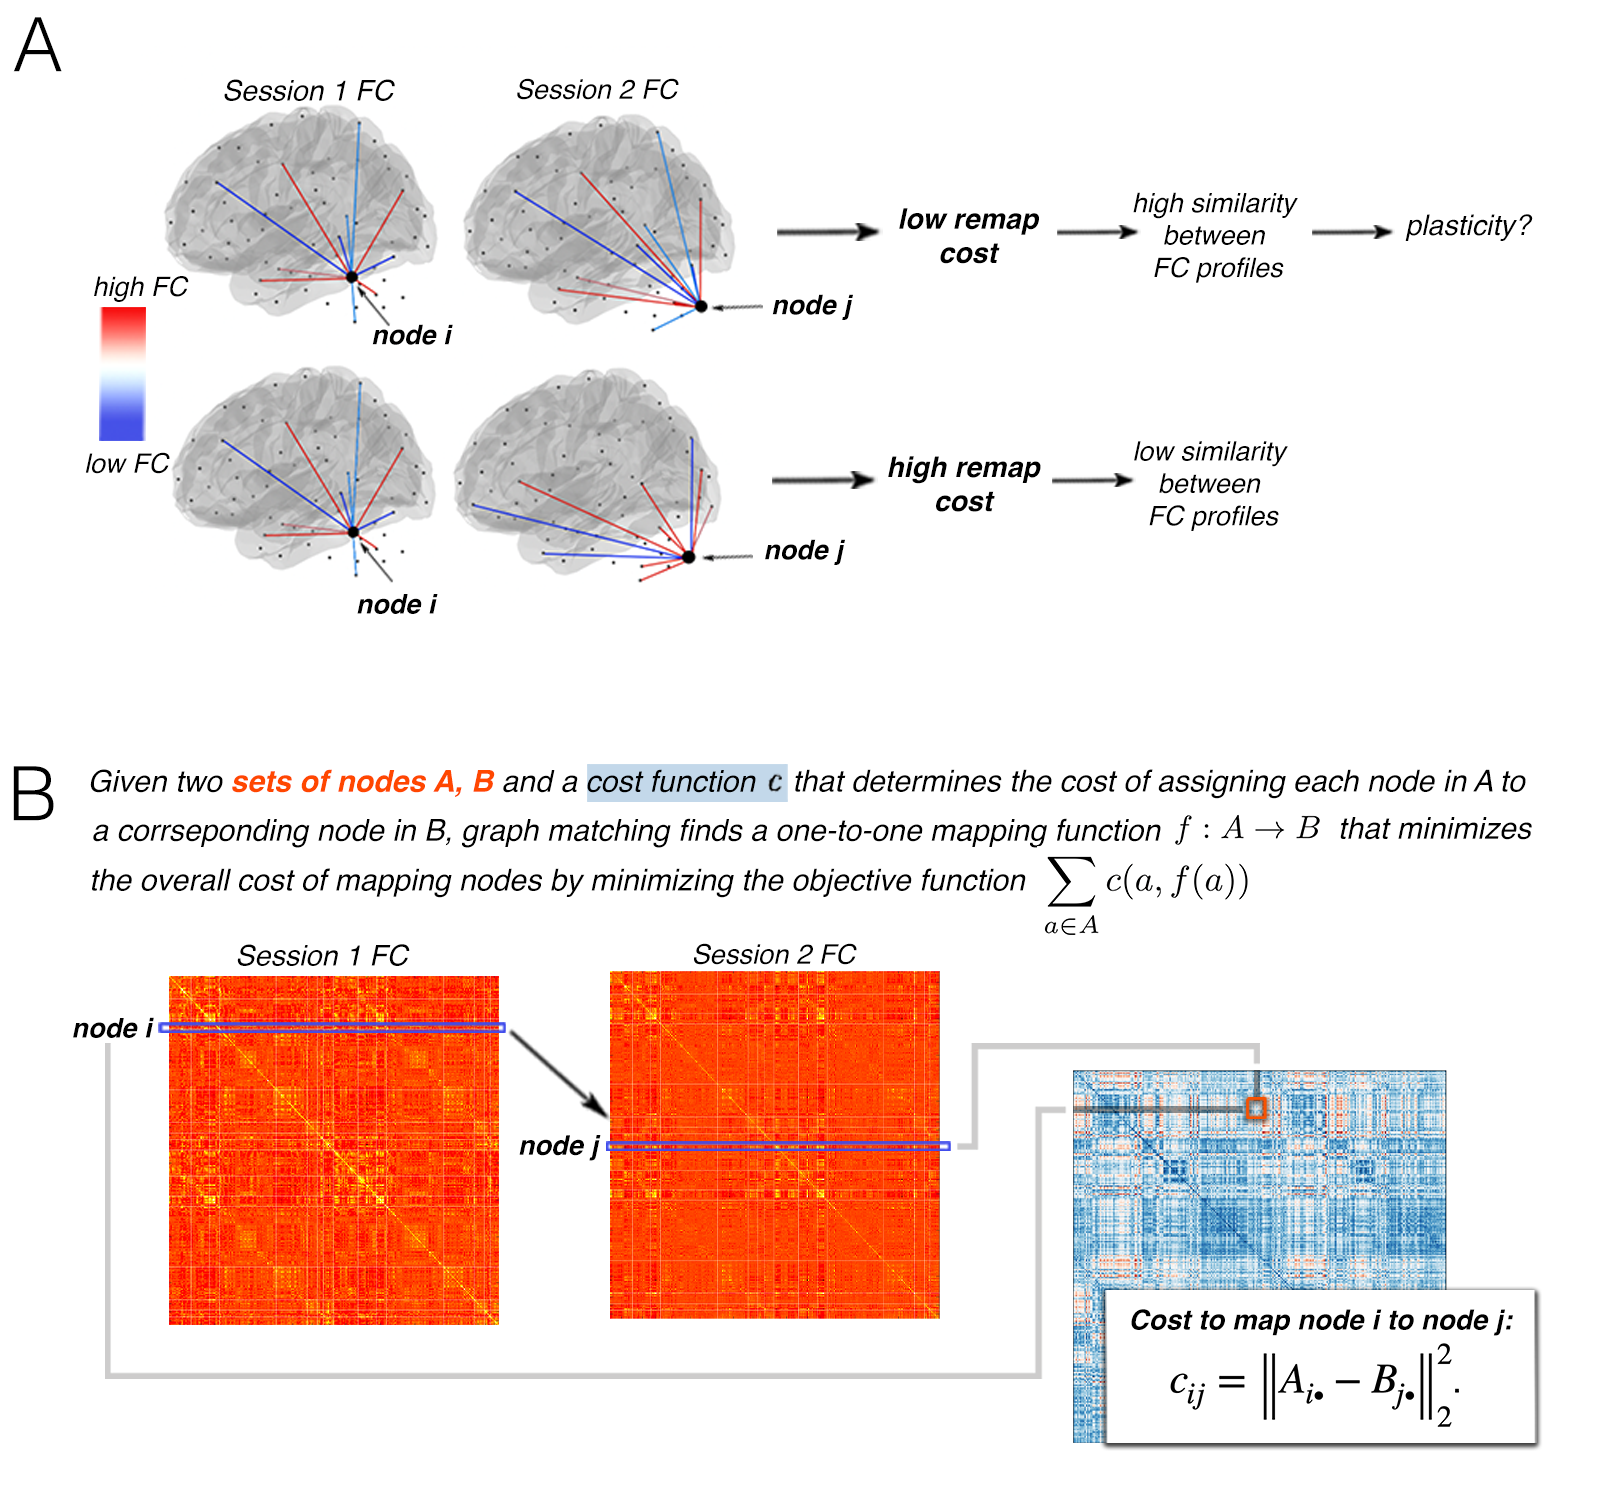
\includegraphics[width=1\textwidth]{graphmatching_procedure.png}
		\caption{Graph matching procedure}
		\centering
	\end{figure}
	
	\subsubsection*{Graph matching}
	We propose the use of graph matching to capture FC network reorganization over time; graph matching has recently been used in brain connectivity networks to map SC to FC \cite{Osmanlioglu2019-ao}. Graph matching is an algorithmic process that maximizes the similarity between two networks by identifying a mapping between similar nodes in the two networks. One approach to identifying the optimal mapping that maximizes the similarity between two networks is with a combinatorial optimization problem known as linear assignment. Take two $n \times n $ networks $A$ and $B$ and a cost function $c: A \times B \rightarrow  \mathbb{R}$  that determines the cost of assigning each node in $A$ to each node in $B$. Here, our cost function is the sum of the entries in the cost matrix $C = \big(c_{i j}\big)$, whose entries are defined by the Euclidean distance between all pairs of rows, representing each node’s FC profile, in $A$ and $B$, i.e. $c_{ij}=|| A_{i\bullet}-B_{\bullet j} ||^2_2$ . In this formulation, the linear assignment problem aims to construct the permutation matrix $P = \big(p_{i j}\big)$ that minimizes the sum of the elements in cost matrix, i.e. $min_P\sum^n_{i=1}\sum^n_{j=1}c_{ij}p_{ij}$. The matrix $P$ is a permutation matrix with exactly one entry equal to 1 in each row and column, and all the rest being zero. Ones in the diagonal mean the same node in the two networks were mapped to one another, while ones in the off-diagonal indicate two different nodes were “remapped” to one another. Here, we will use the Hungarian algorithm to solve this minimization problem and find the corresponding optimal permutation matrix  Figure 1 illustrates how the graph matching will be applied to subsequent longitudinal FC networks (from 1 week to 1 month and 1 month to 6 months) from each stroke and control individual. In the top row of Figure 1 the two brain regions (black spheres, labeled node i and node j) have very similar functional profiles, depicted with red and blue lines to other regions, and thus the cost of remapping them is low. In the second row of Figure 8A, the two brain regions have very different functional profiles and thus the cost of remapping them is high. An example cost matrix from a stroke subject’s FC extracted from 1 week MRI and FC extracted from 1 month MRI is provided in Figure 8B. Unsurprisingly, the lowest costs are along the diagonal (the same region mapping to itself between time points) and across left-right homologues (in the prominent super and sub diagonals).

	\subsubsection*{Estimation of functional reorganization}
	The permutation matrices calculated for each pair of time points for each individual were used as a measure of functional reorganization. To assess the spatial pattern of reorganization, the number of times each node was remapped across all subjects was calculated as the 'remap frequency’, where nodes with a greater remap frequency are assigned to alternative nodes in the subsequent time point. For each subject the number nodes that were remapped can be calculated as a subject-specific measure of the extent of functional reorganization. Inspection of the patterns in the off-diagonal allows for identification of region pairs that may be remapping over time.
	
	\subsubsection*{Code availability}
	 The code for partial functional connectivity calculation, graph matching, and remap frequency is available on GitHub: https://github.com/emilyolafson/stroke-graph-matching
	
	\section*{Results}
	\subsubsection*{Brain areas with greater structural disruption reorganize more frequently}
	Functional remapping frequency scores were highest in the brainstem and cerebellum, and to a lesser extent in the motor cortices (Figure 2a), similar to the spatial distribution of ChaCo (structural disconnection) scores, which were also highest in the brainstem and cerebellum (Supplementary Figure). For each pair of longitudinal, subsequent time points, there was a significant, positive correlation between average regional ChaCo scores across subject and functional remapping frequency, indicating those regions with more baseline structural connectivity disruption also had more remapping over time (Figure 2b).
	Furthermore, for about 50 percent of subjects, the nodes that remap have significantly higher ChaCo scores compared to those that do not remap (Supplementary fig) and the t-statistic is positive for non-significant p-values. 


	\begin{figure}[ht]
		\begin{subfigure}{.5\textwidth}
			\centering
			% include first image
			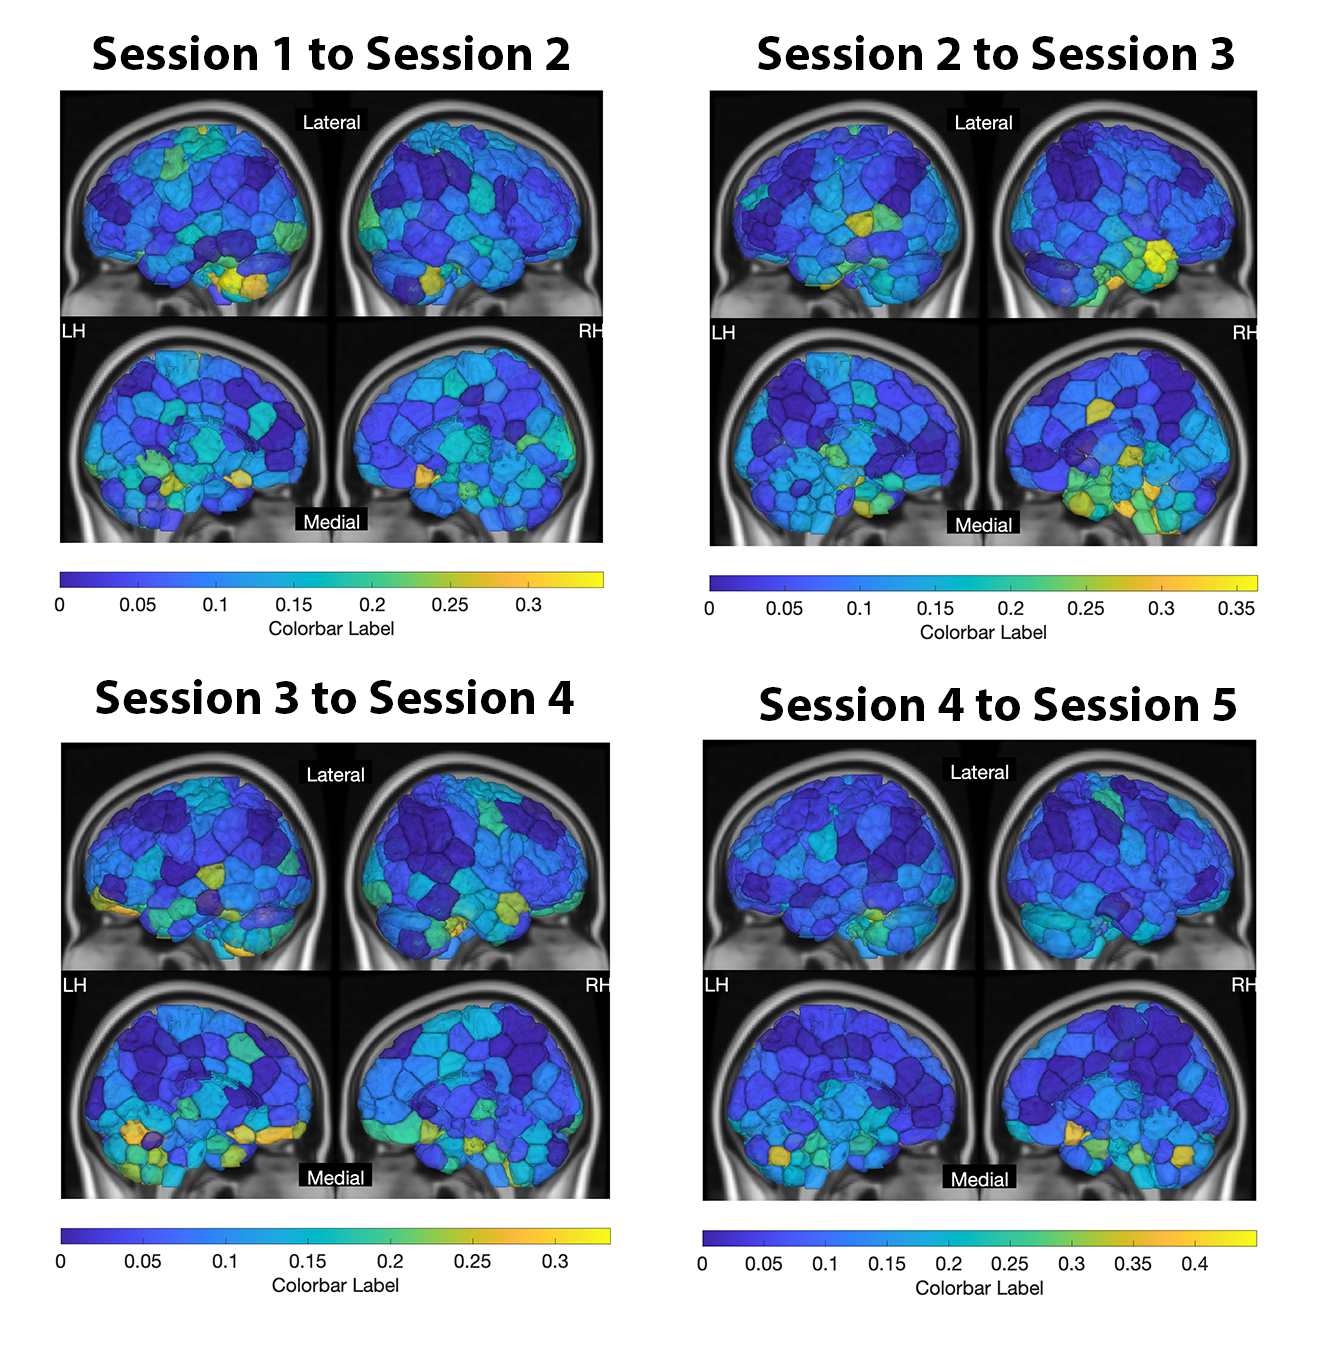
\includegraphics[width=1\linewidth]{gummi_remapfreq_allsessions.png}  

			\label{fig:sub-first}
		\end{subfigure}
		\begin{subfigure}{.5\textwidth}
			\centering
			%  second image
			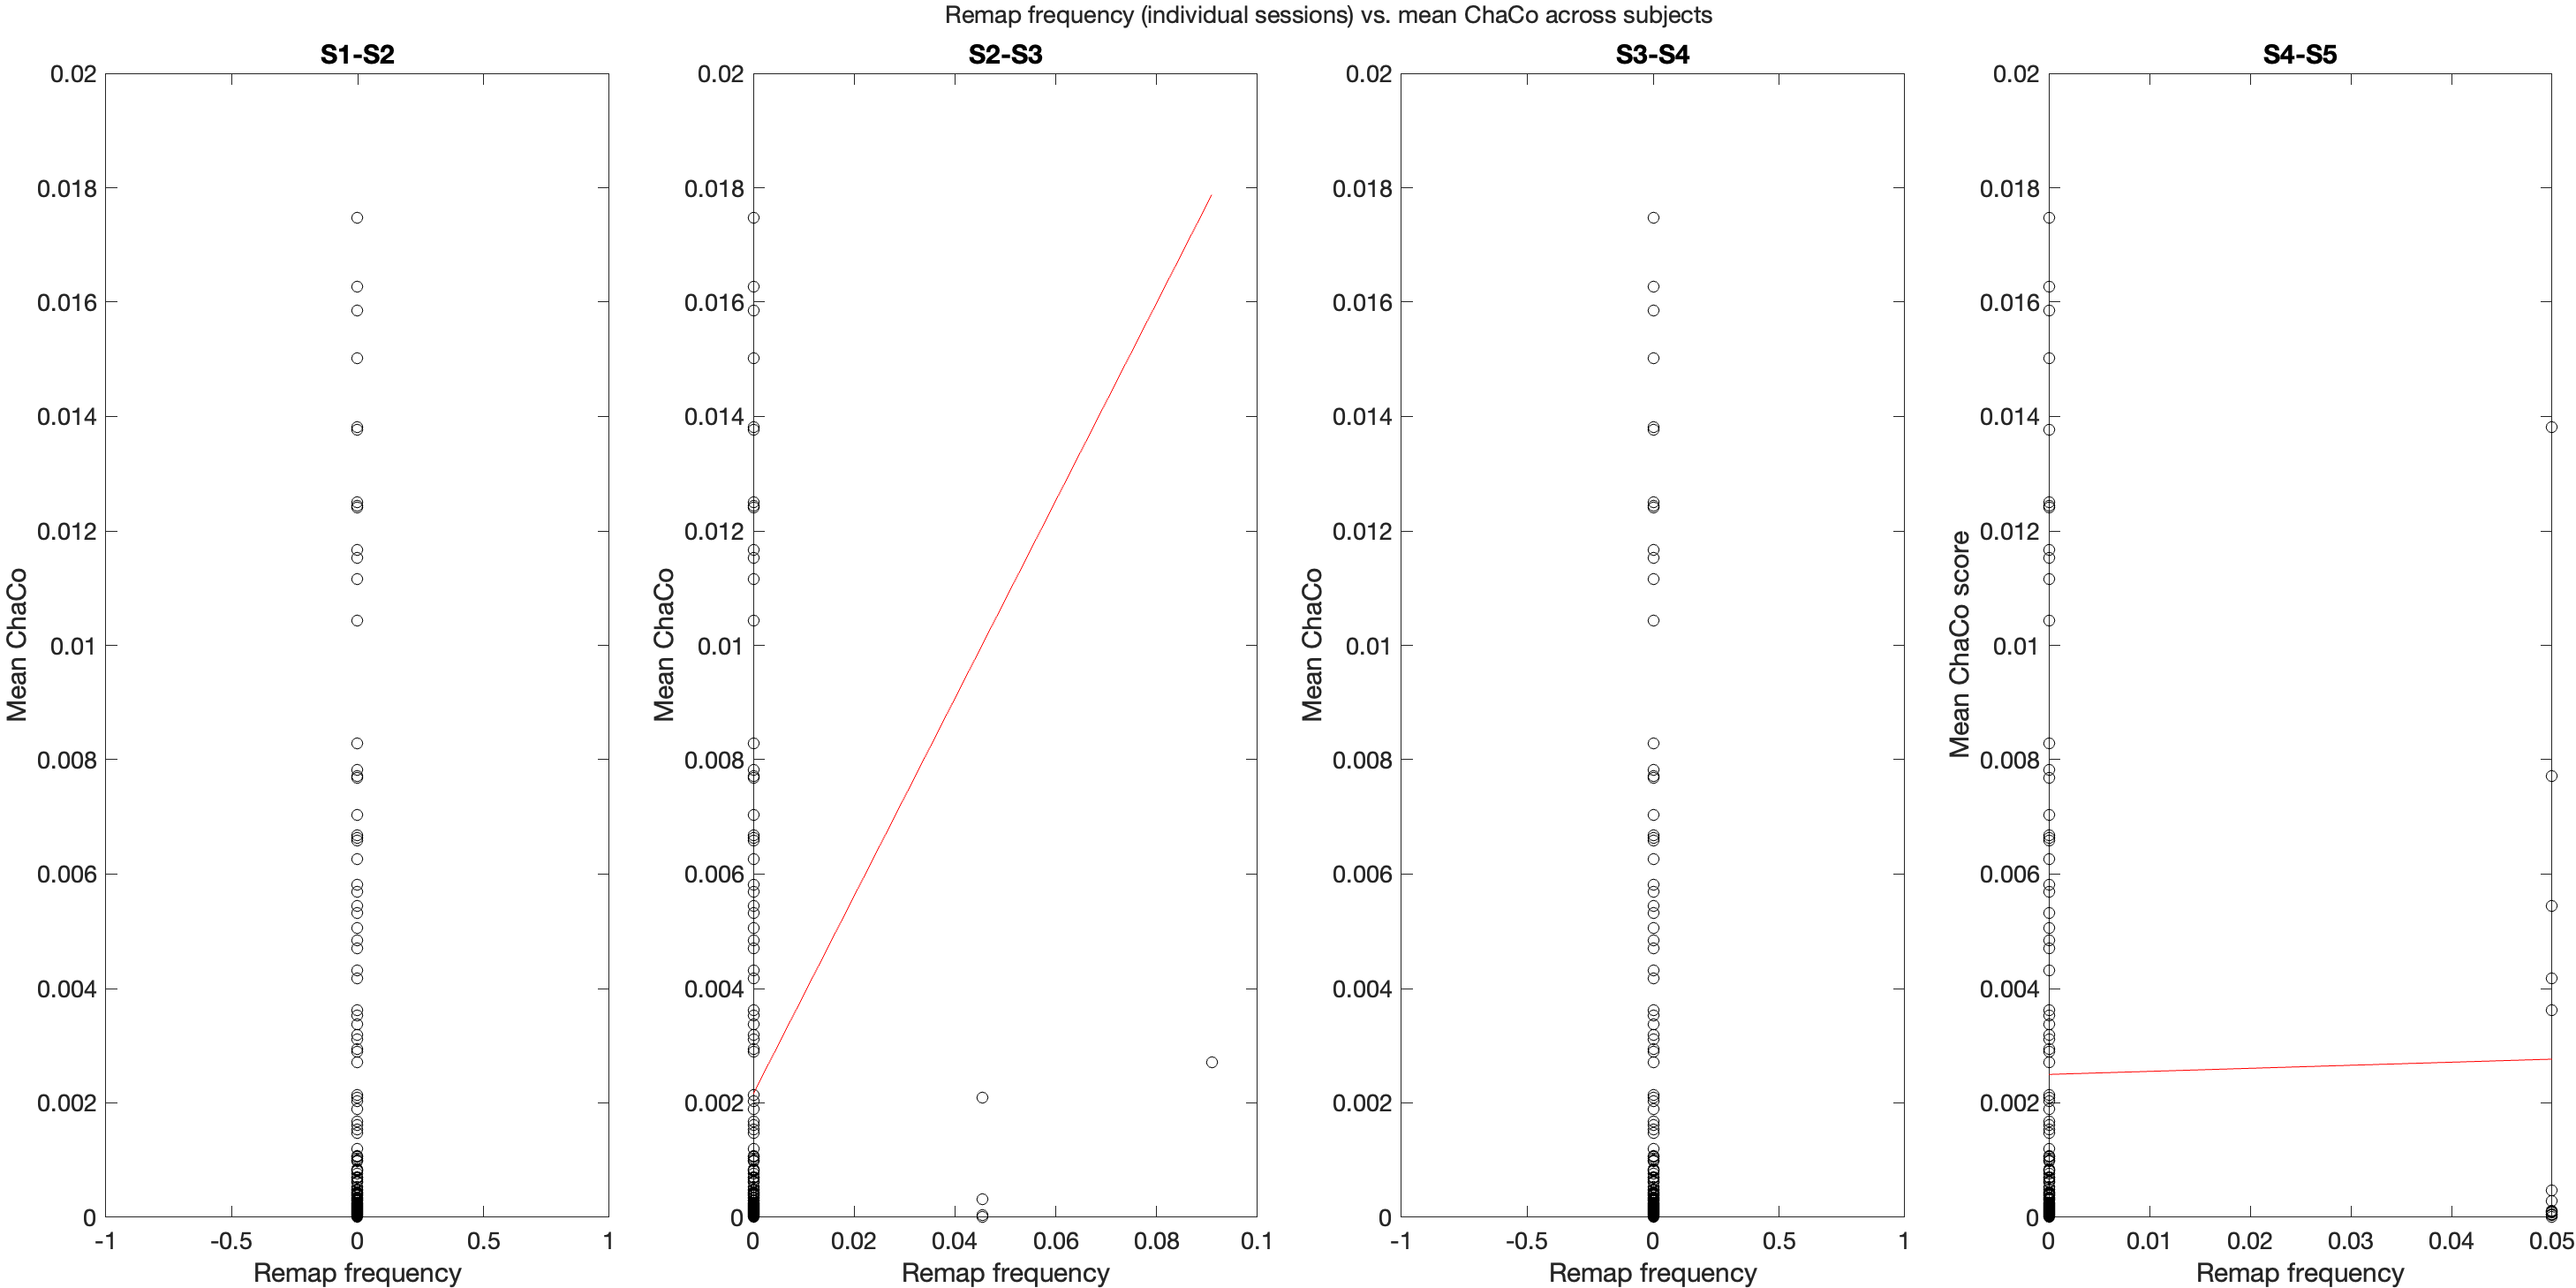
\includegraphics[width=1\linewidth]{corr_remapping_chaco.png}  

			\label{fig:sub-second}
		\end{subfigure}
	\end{figure}



	\begin{figure}
		\begin{subfigure}{.5\textwidth}
			\centering
			%  third image
			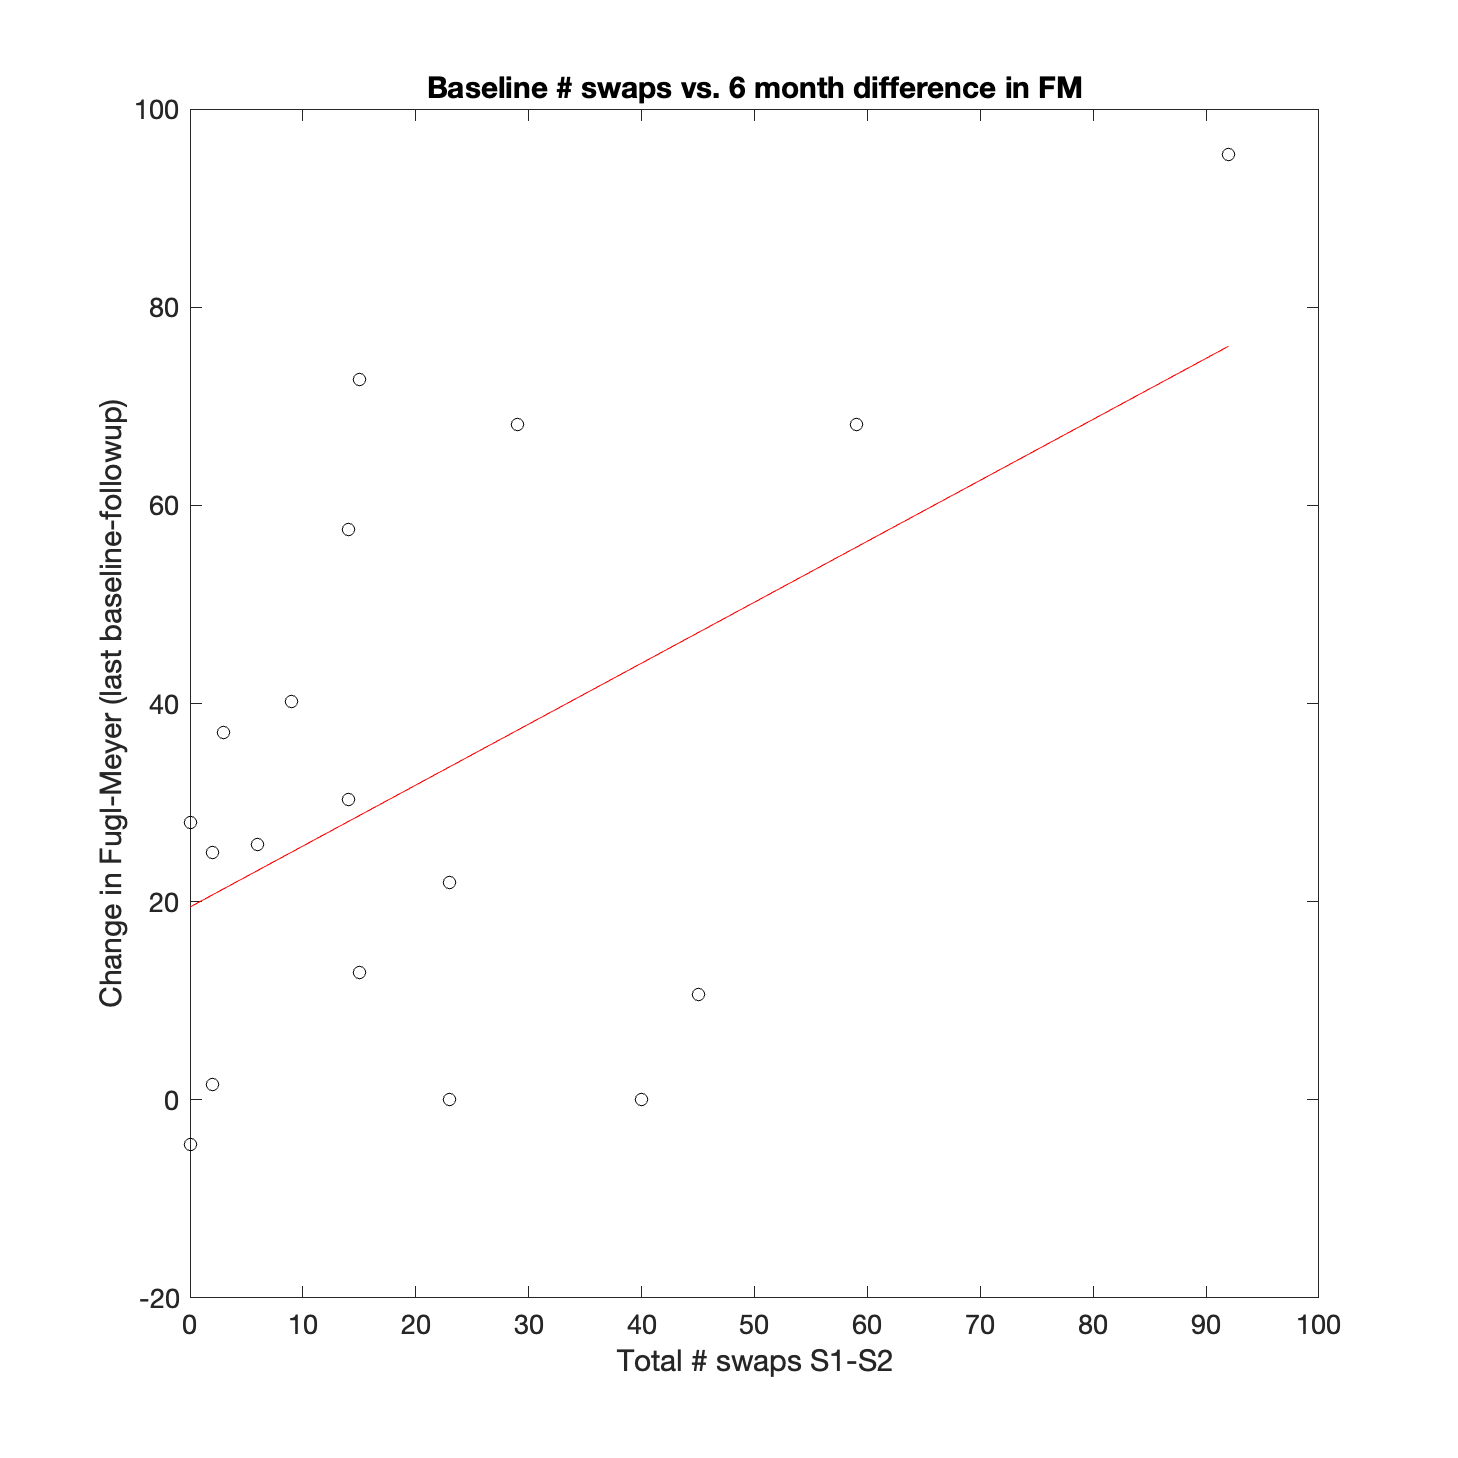
\includegraphics[width=1\linewidth]{baselineswaps_6monthFM.png}  

			\label{fig:sub-second}
		\end{subfigure}
		\begin{subfigure}{.5\textwidth}
			\centering
			%  fourth image
			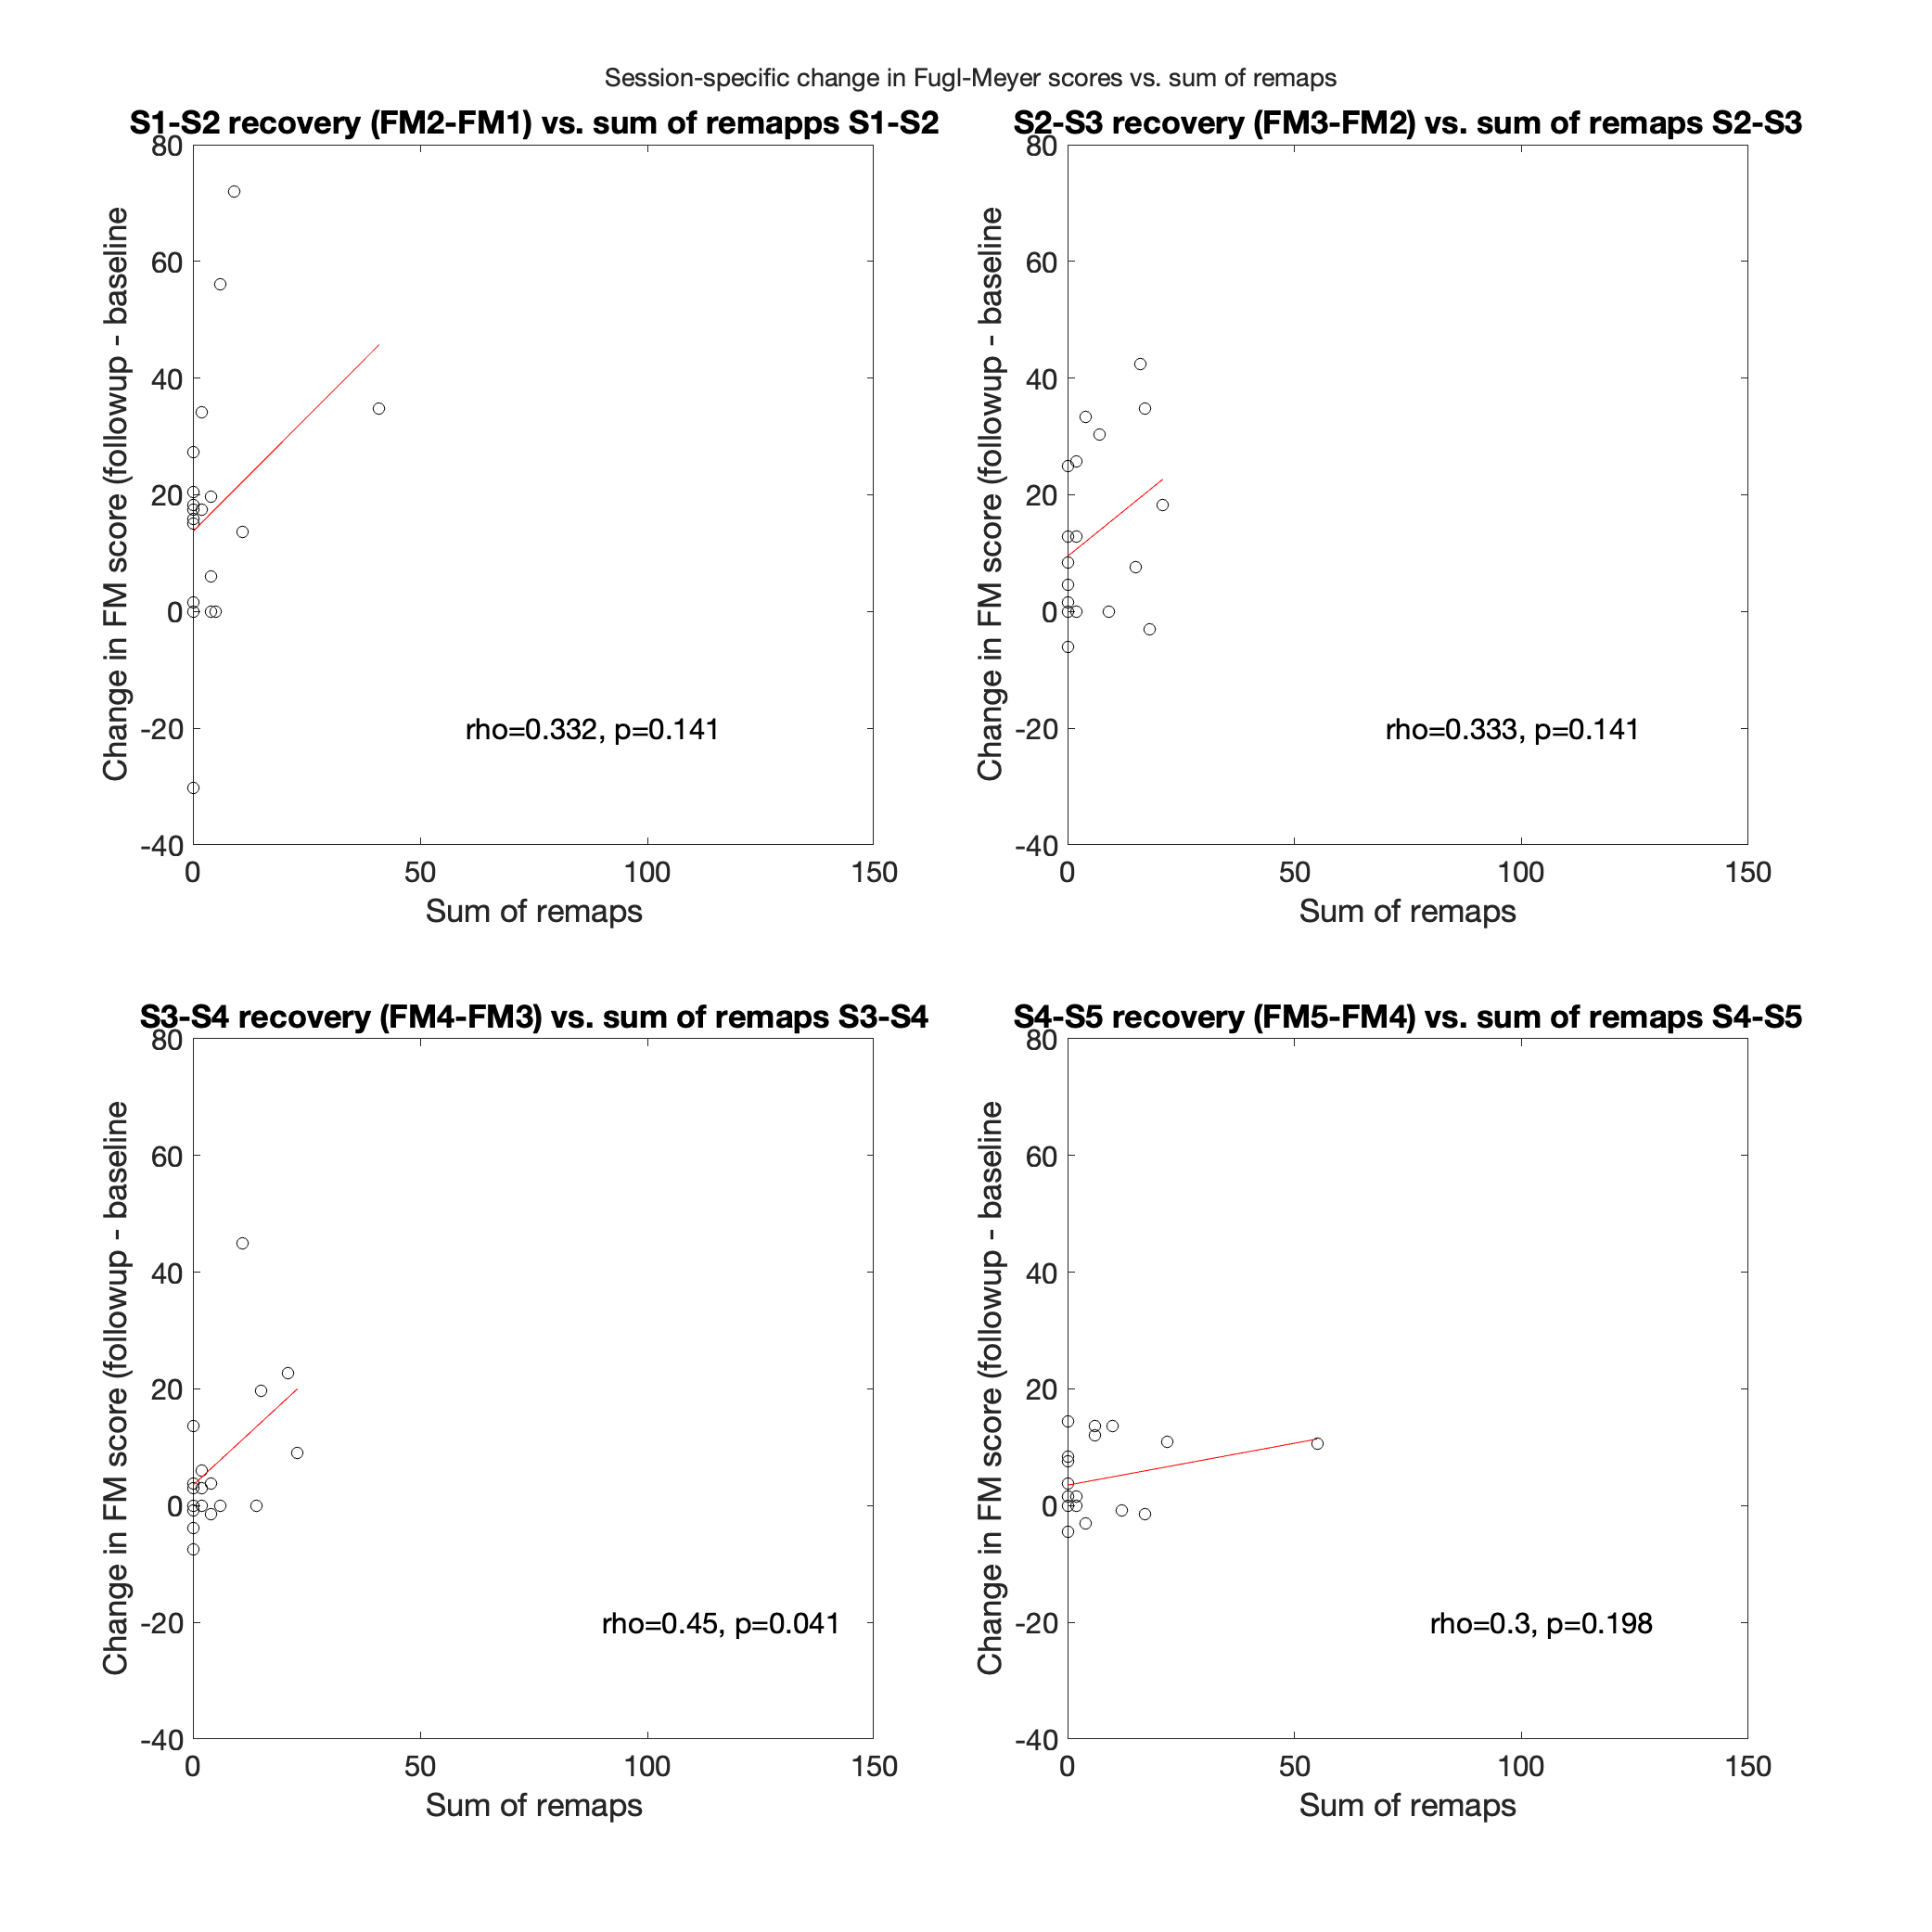
\includegraphics[width=1\linewidth]{remaps_recovery_sessionspecific.png}  
			\label{fig:sub-second}
		\end{subfigure}
		\caption{Put your caption here}
		\label{fig:fig}
	\end{figure}
	The impact of noise from lesions on the underlying BOLD signal is likely not driving remapping, as the maximum overlap of the lesions with each ROI is maximum 30 percent (Supplementary fig) and the average percent lesion overlap with each ROI across subjects does not correlate with remap frequency (Supplementary fig). Lesion size is also unrelated to the number of remaps for each subject, but the lesion load on the corticospinal tract (Supplementary methods) does significantly positively correlate with the amount of reorganization between session 1 and 2 (Supplementary fig). We also found that the number of remaps was not related to motion as measured by framewise displacement (Supplementary Fig).
	
	and do the same analysis in controls to show that the t-stat distribution is near 0/not positive
	Nodes that remap in controls (?) are not the same nodes that remap in stroke subjects and do not correlate with stroke group average ChaCo scores (Supplementary Fig)
	
	\subsubsection*{Amount of functional reorganization is related to impairment and recovery}
	We observed a significant positive correlation between baseline impairment, as measured by the Fugl-Meyer assessment, and the number of remaps, such that patients who were more impaired at 7 days post-stroke had more remapping over the second week post-stroke (day 7 to day 14) (Fig 3). 
	

	\section*{Discussion}
	
	\section*{Supplementary}
	\subsection*{Supplementary Methods}
	\subsection*{Supplementary Figures}
	
	\begin{figure}[h]
		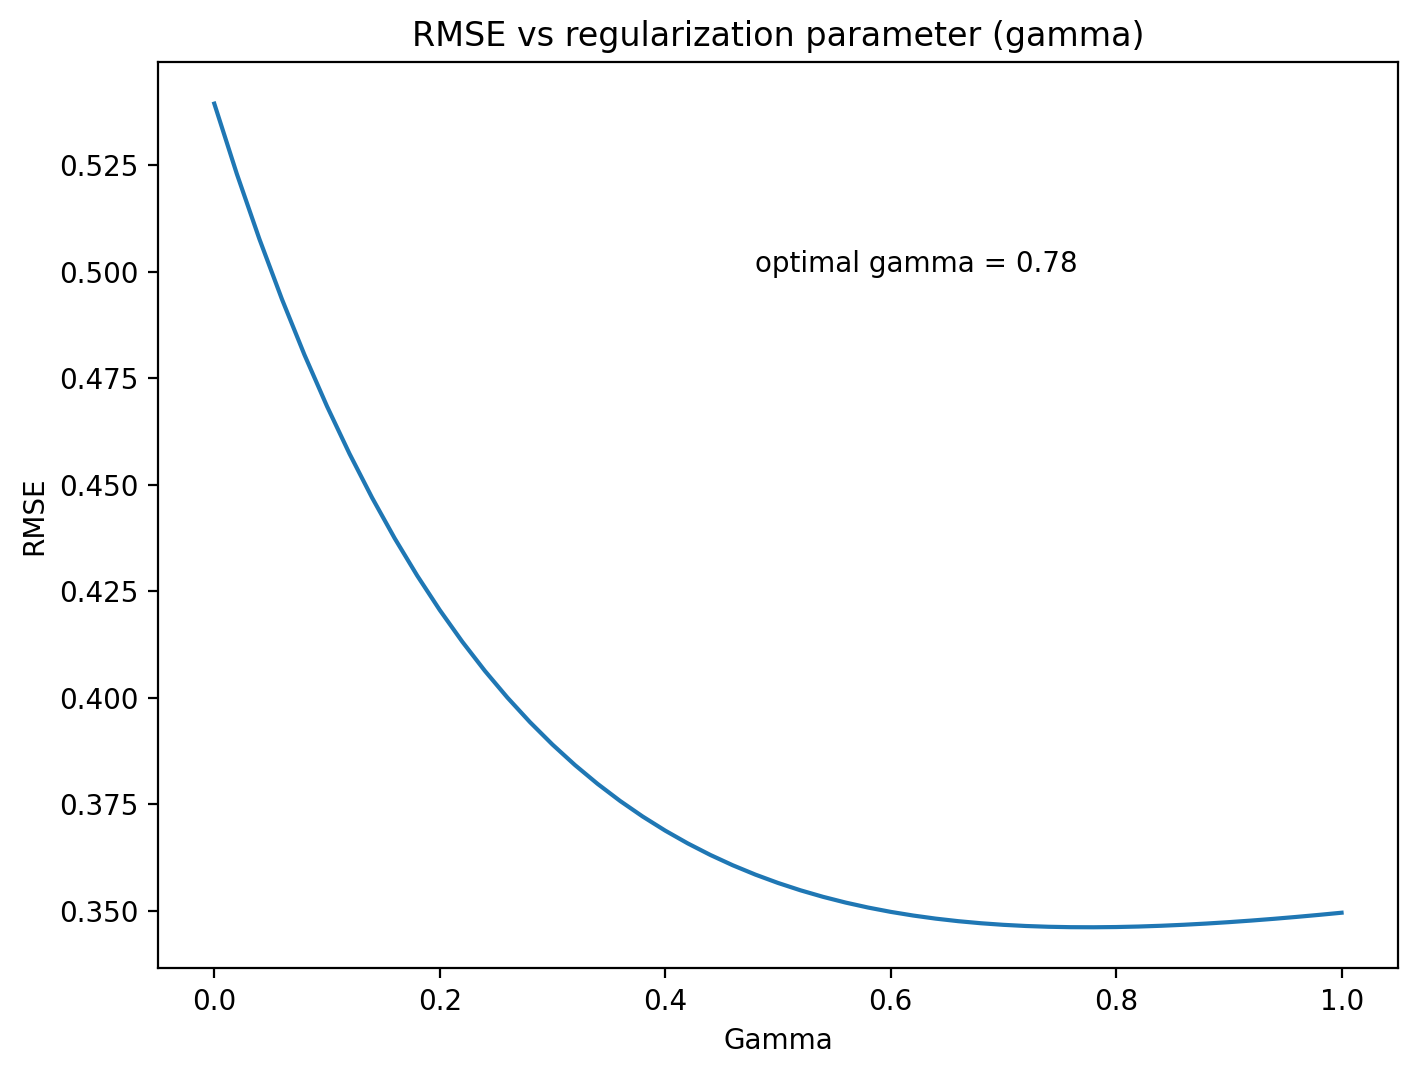
\includegraphics[width=0.9\textwidth]{precision_fullFCs.png}
		\caption{Results of gridsearch for gamma; plotted is the root mean squared error (RMSE) across subjects of the norm of each subject's precision matrix and the group avergae unregularized precision matrix at each lambda. The optimal gamma that minimized the RMSE across subjects was 0.78}
				\centering
	\end{figure}

	\begin{figure}[h]
	\includegraphics[width=0.9\textwidth]{allsubjects_chaco.pdf}
	\caption{ChaCo scores of all subjects}
	\centering
	\end{figure}

	\begin{figure}[h]
	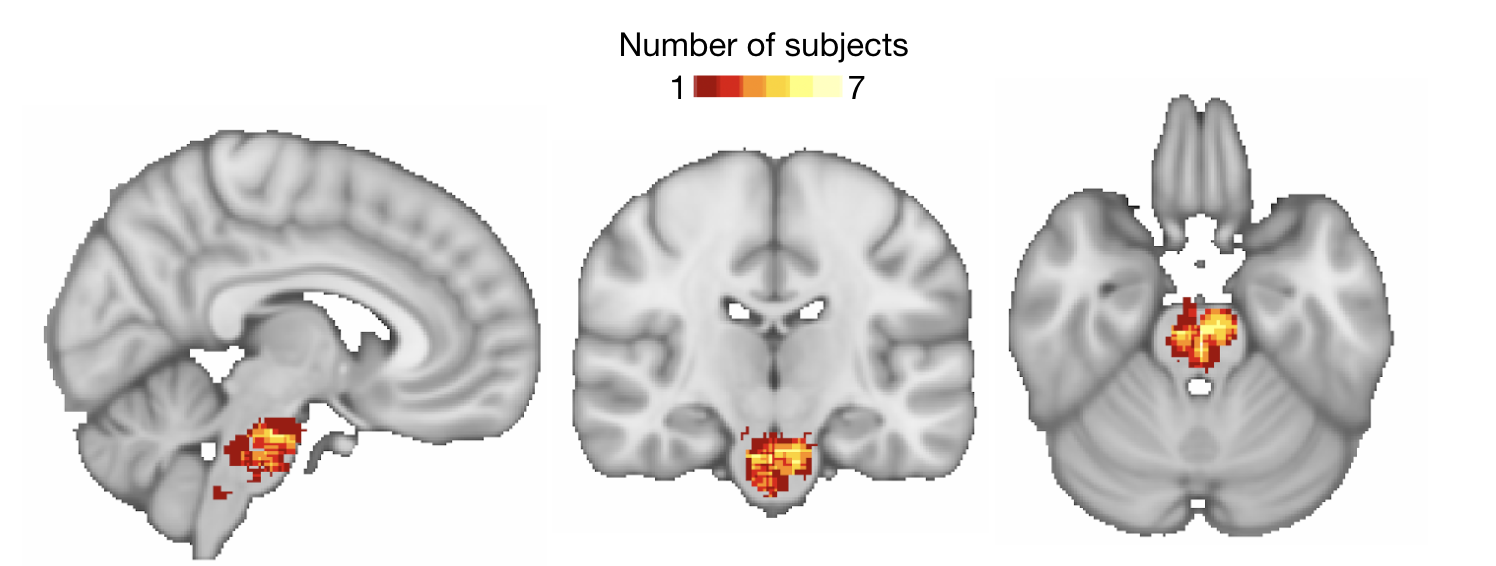
\includegraphics[width=0.9\textwidth]{lesioncount.png}
	\caption{Distribution of lesions across all subjects.}
	\centering
	\end{figure}

	\begin{figure}[h]
	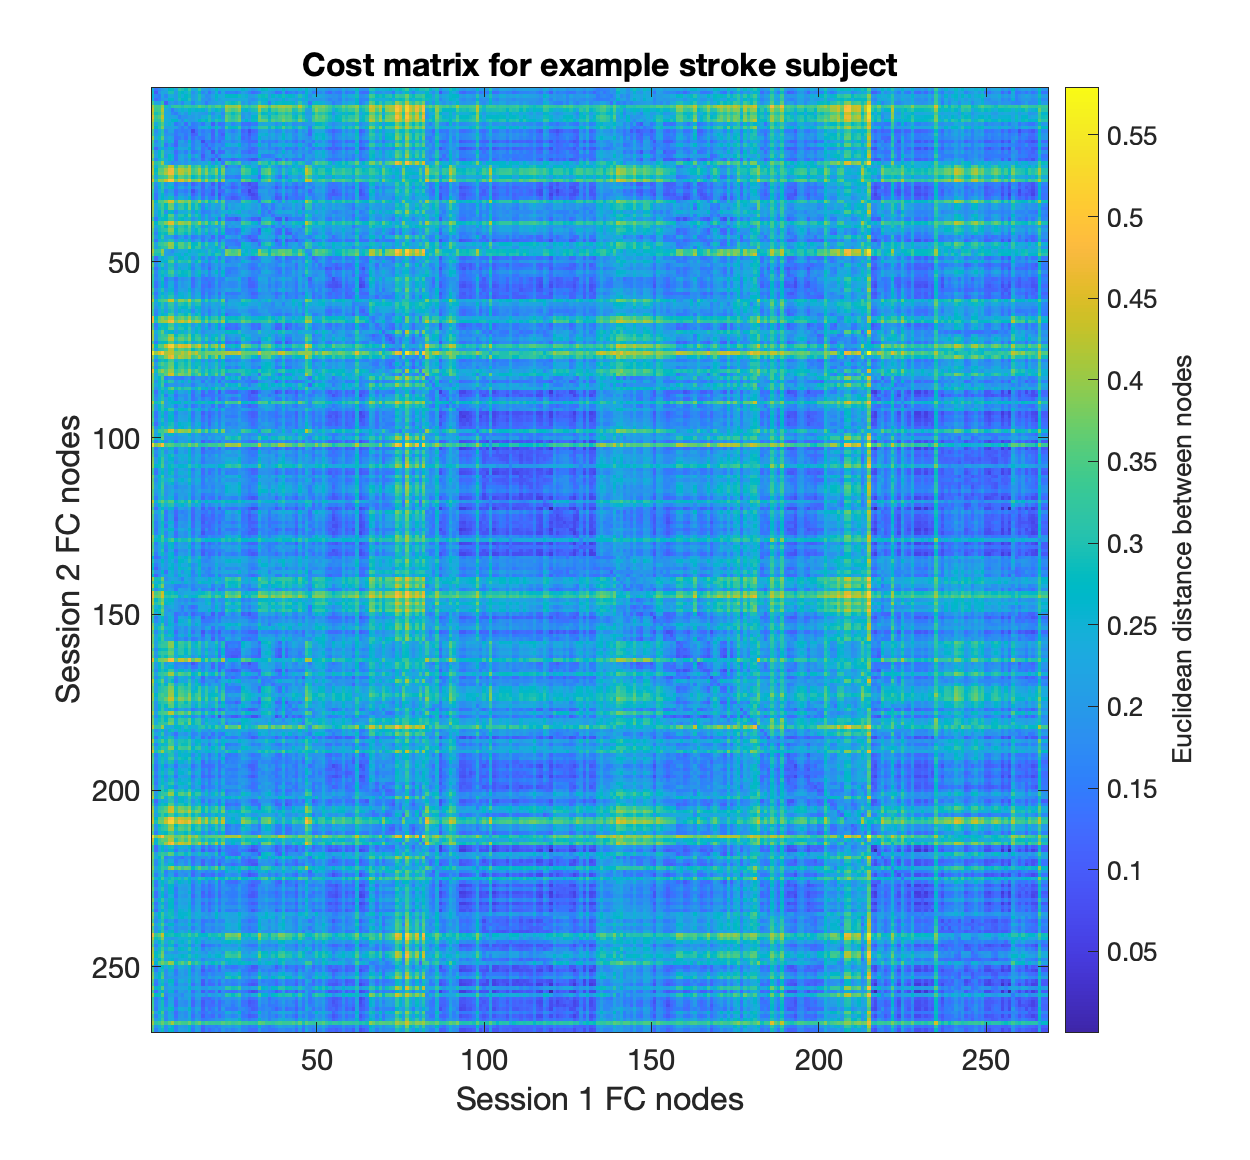
\includegraphics[width=0.9\textwidth]{costmat.png}
	\caption{Cost matrix indicating the cost of remapping nodes from session 2 (vertical axis) to every other node in session 1 (horizontal axis).}
	\centering
	\end{figure}

	\begin{figure}[h]
	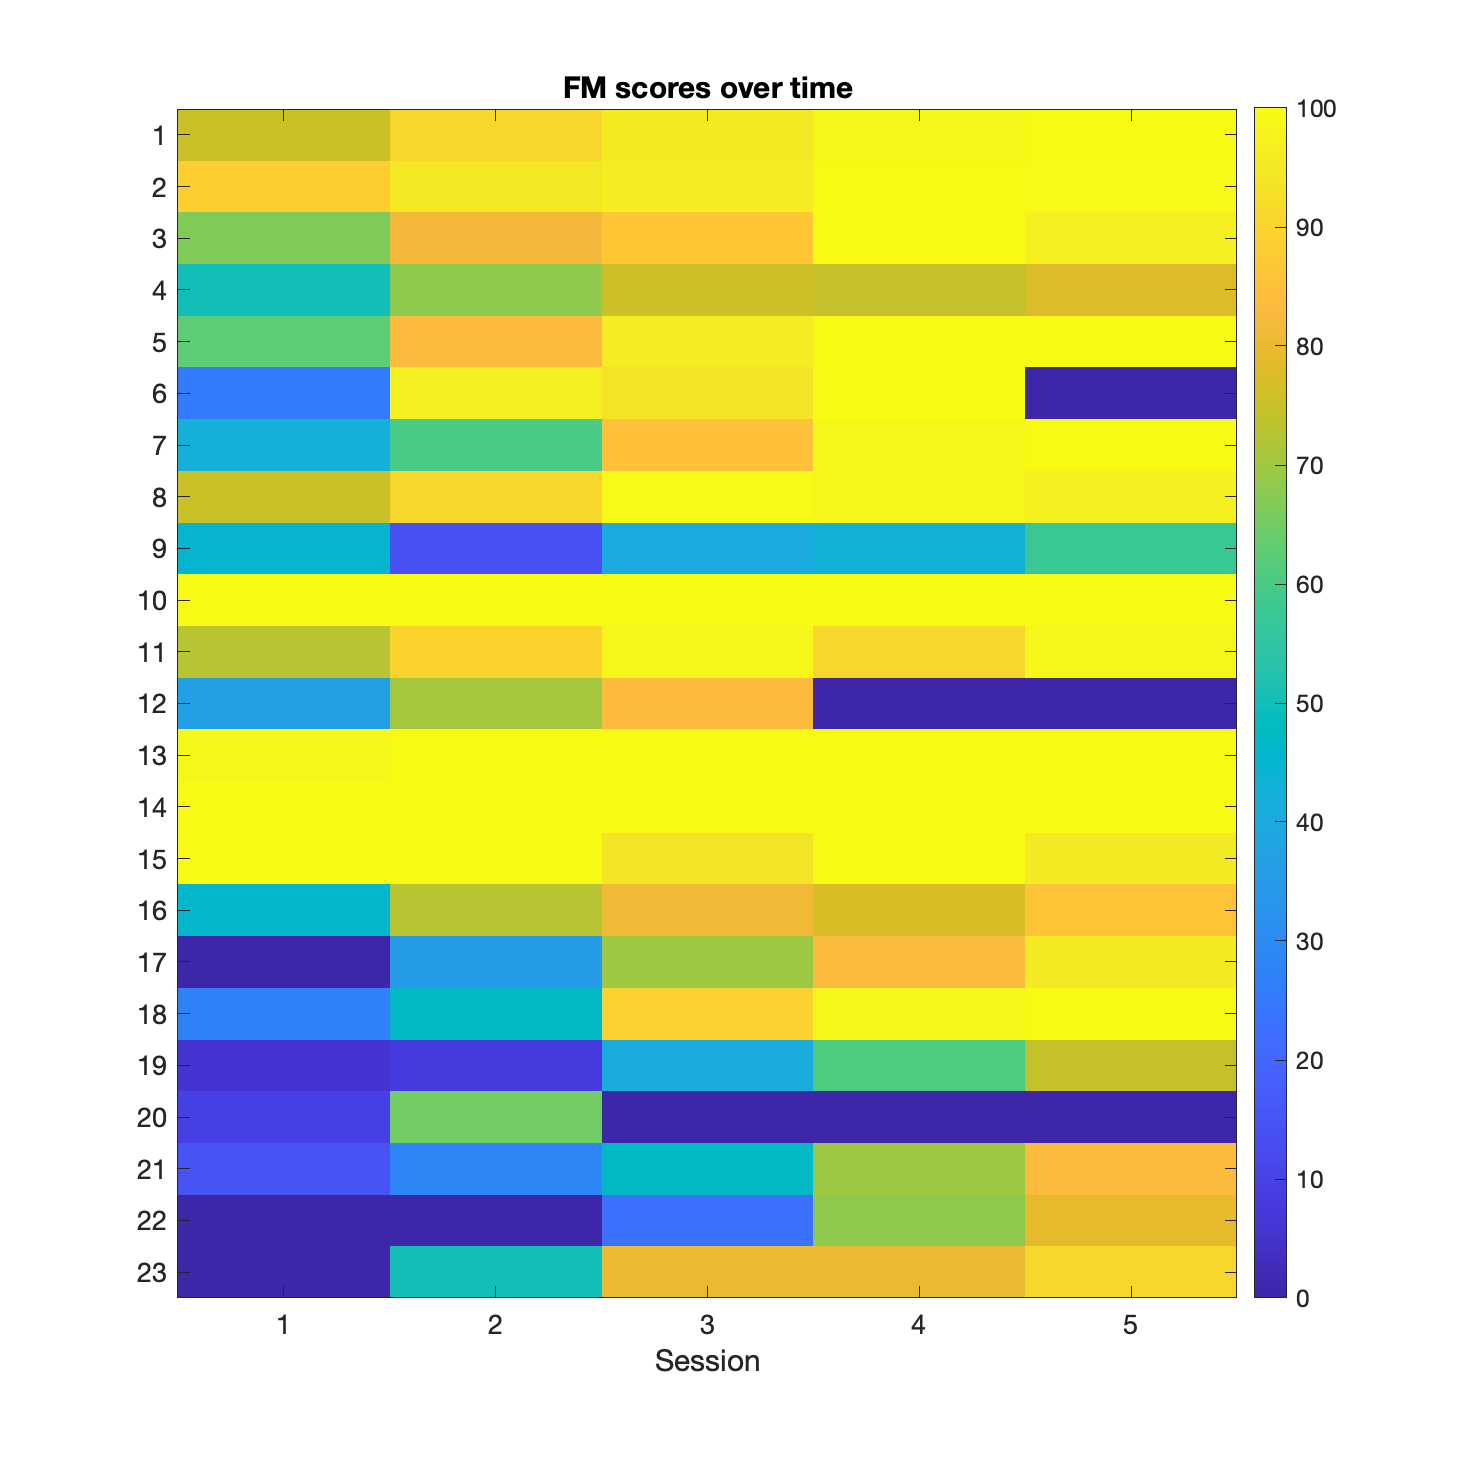
\includegraphics[width=0.9\textwidth]{FM_overtime.png}
	\caption{Fugl-Meyer scores for all subjects over sessions. Note that for subjects 6, 12, 20, 22, and 23 several scores are missing.}	\centering
	\end{figure}


	\begin{figure}[h]
	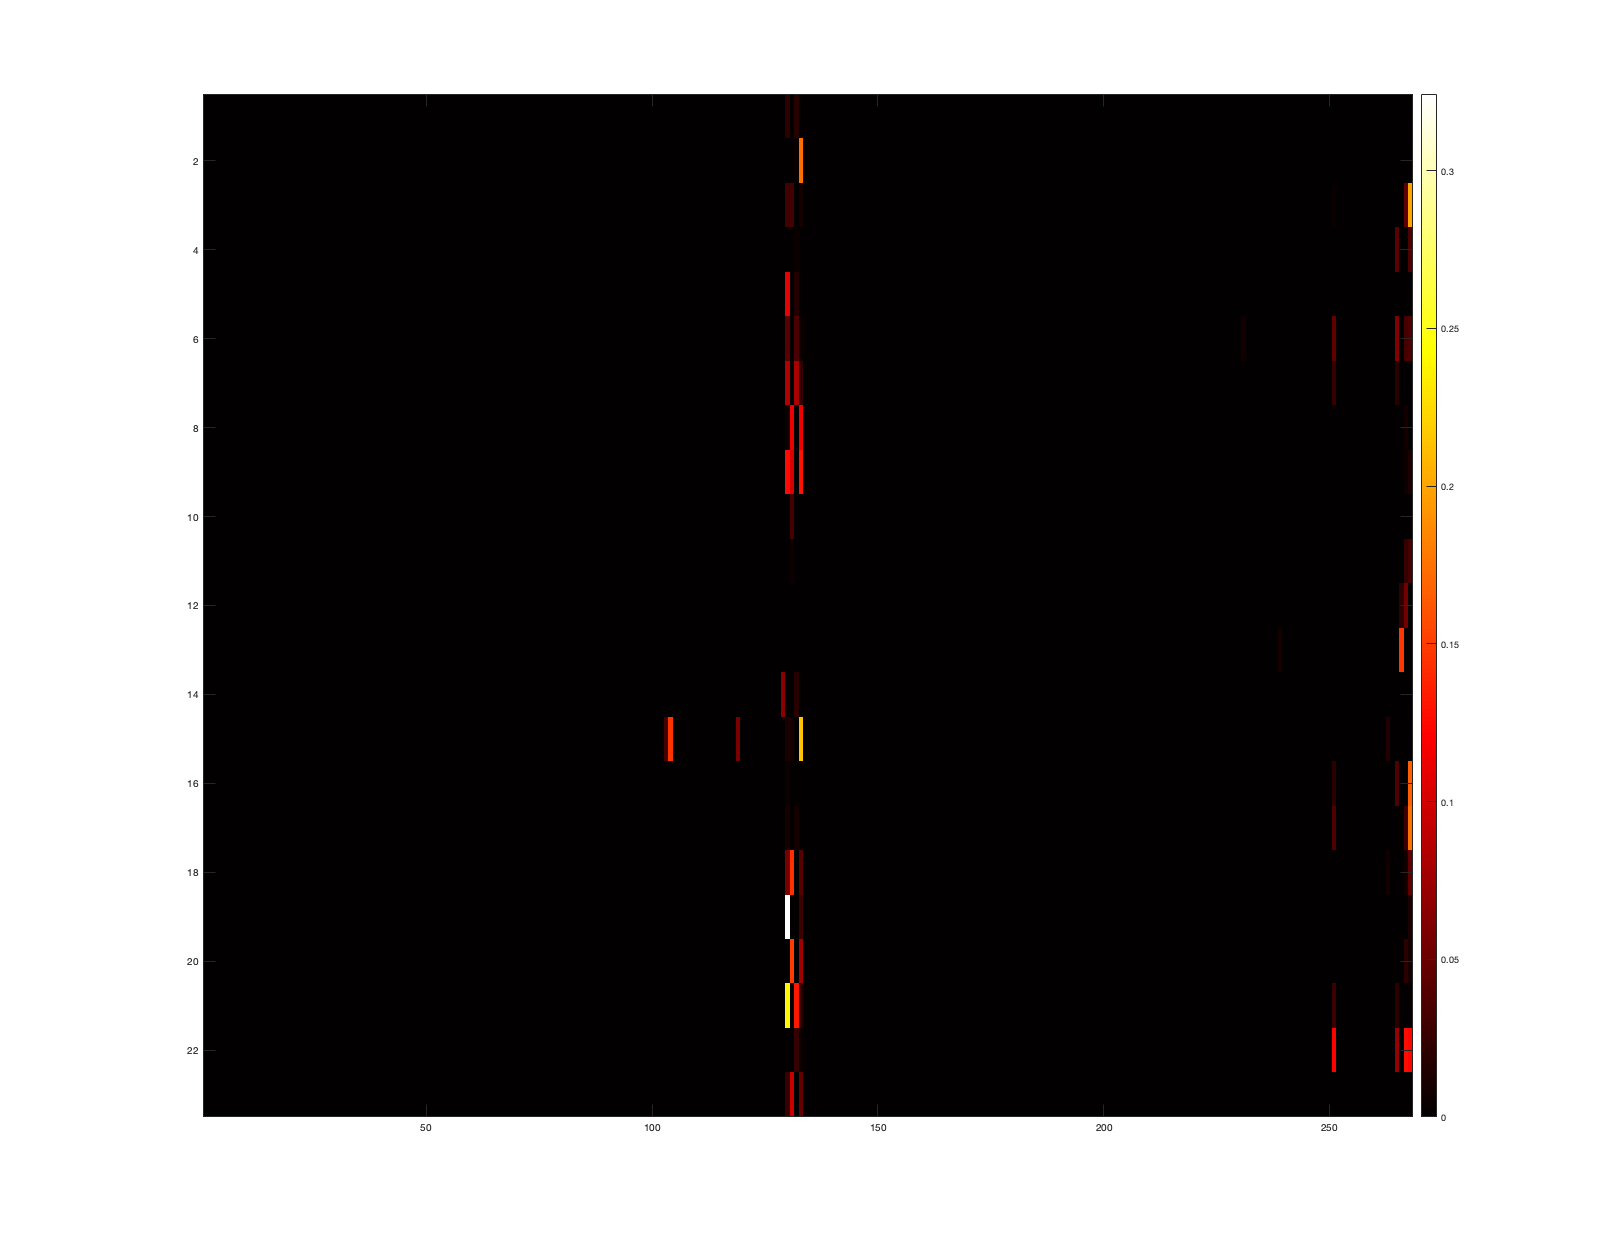
\includegraphics[width=0.9\textwidth]{proportion_overlap_w_lesion.png}
	\caption{Extent of overlap between each of the 268 ROIs}	\centering
	\end{figure}

	\begin{figure}[h]
		\begin{subfigure}{.5\textwidth}
		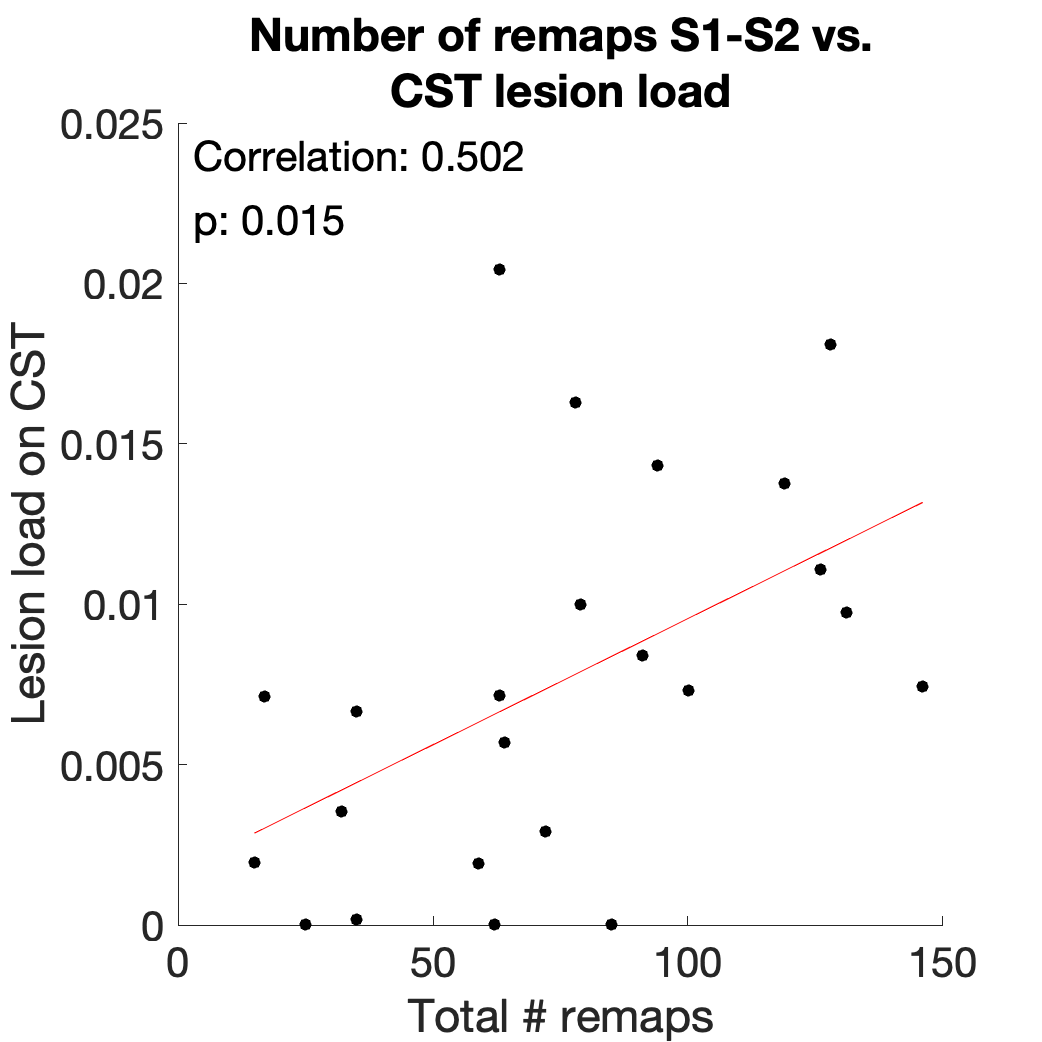
\includegraphics[width=1\textwidth]{lesionload_remapss1s2.png}
		\caption{Lesion load on the CST calculated as the proportion of the CST that intersects with the binary lesion mask (calculated on the ipsilesional CST)}
		\centering
		\end{subfigure}
		\begin{subfigure}{.5\textwidth}
		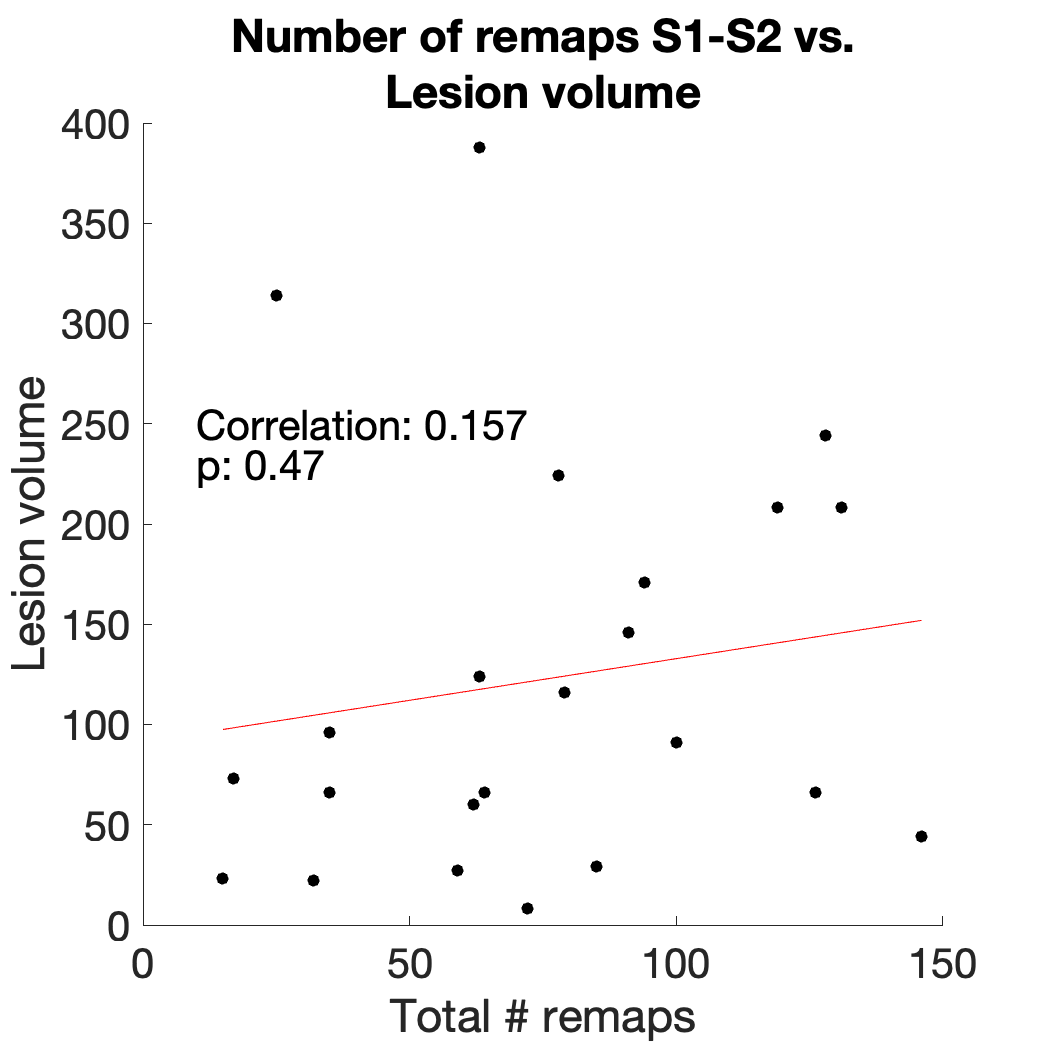
\includegraphics[width=1\textwidth]{lesionvol_remapss1s2.png}
		\caption{Lesion volume in mm$^{3}$}
		\centering
		\end{subfigure}
	\label{fig:fig}
	\end{figure}
	%----------			-----------------------------------------------------------
	\section*{Bibliography}

	\printbibliography

	
\end{document}
